% RESULTADOS-------------------------------------------------------------------

\chapter{RESULTADOS}
\label{chap:resultados}

Este capítulo ilustra como foram feitas as etapas de implementação, detalhando alguns fatores importantes nos códigos utilizados, métodos para a descoberta ótima do número de focos para cada base,
assim como uma breve explicação sobre as bases de dados utilizadas e algunas das métricas empregadas. Também apresenta os resultados
obtidos, e análises pertinentes a estes resultados, estabelecendo um comparativo com as técnicas convencionais de pesquisa por similaridade. Todos os resultados foram extraídos utilizando o SGBD
PostgreSQL 10.3 em conjunto com o aplicativo pgAdmin 4 versão 2.1, responsável pela interface com o banco de dados. O hardware utilizado para as pesquisas é um Intel® Core i7™ 7700HQ 2.8 GHz possuindo 16 GB de memória RAM.
O sistema operacional utilizado foi o Windows 10 Home Edition.


\section{BASES DE DADOS}
\label{sec:basesdedados}
Foram utilizadas duas bases de dados complexas distintas para a verificação deste trabalho: uma base de imagens de cães e gatos, e uma
base de dados extraídos de exames médicos de imagem.

\catcode`\_=13 
\def_{\textunderscore}
\subsection{BASE CAT_DOG}
\catcode`_=8
\label{subsec:catdog}
Esta base de dados é dividida entre conjunto de teste e conjunto de treinamento, e encontra-se disponível em \href{https://www.kaggle.com/c/dogs-vs-cats}{<https://www.kaggle.com/c/dogs-vs-cats>}.
A base originalmente foi criada para uma competição promovida pela comunidade de cientistas de dados conhecida como Kaggle, aonde o objetivo era criar o algoritmo que conseguisse classificar imagens
entre fotografias ou desenhos de gatos ou cachorros com o maior índice de acerto. 

Para a verificação da técnica implementada, foi utilizado o conjunto de imagens de treino, com 25000 imagens, divididas igualmente entre cães e gatos. 
Tornou-se necessário a remoção de 3 imagens que eram pequenas demais e impossibilitavam a segmentação destas na etapa de processamento de imagens. As imagens foram processadas para a extração
das características desejadas e inseridas no banco de dados. As características escolhidas para cor foram a média e a variância do valor dos pixels em cada um dos três canais, para textura
foram dissimilaridade, contraste e correlação, e para a característica de forma foram utilizadas métricas como área, excentricidade e a razão área sobre área convexa. Todas as características
foram extraídas utilizando um script feito na linguagem Python versão 3.5, com o auxílio da biblioteca de algoritmos de manipulação de imagens \textit{scikit-image}.
\begin{figure}[H]
  \centering
  \subfloat[cat.325]{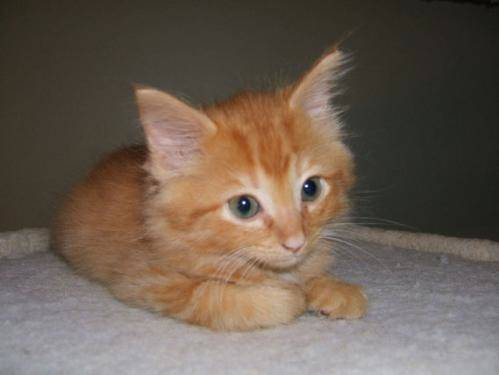
\includegraphics[width=.20\textwidth]{dados/figuras/cat325.jpg}} \hspace{2cm}
  \subfloat[cat.6243]{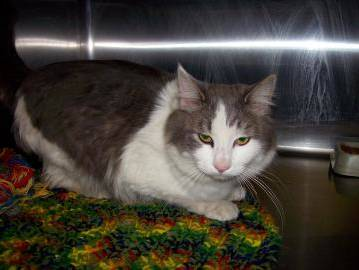
\includegraphics[width=.20\textwidth]{dados/figuras/cat6243.jpg}} \\
  \subfloat[dog.2032]{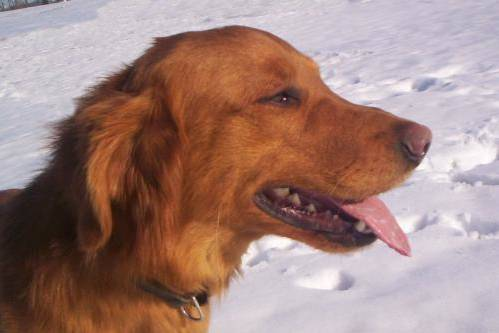
\includegraphics[width=.20\textwidth]{dados/figuras/dog2032.jpg}}\hspace{2cm}
  \subfloat[dog.10641]{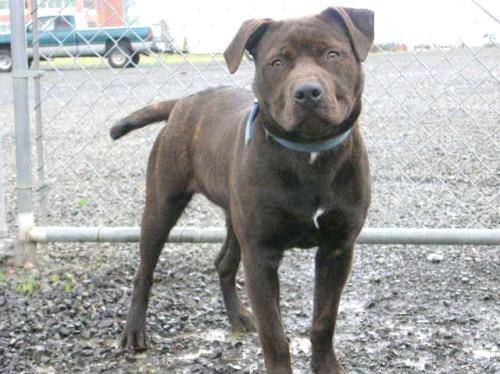
\includegraphics[width=.20\textwidth]{dados/figuras/dog10641.jpg}} 
  \caption{Exemplos de imagens da base CAT\_DOG}
\label{fig:catdogex}
\end{figure}

\subsection{BASE HC}

A base HC foi fornecida pelo Hospital das Clínicas de Ribeirão Preto, e ela consiste em 500000 imagens com as suas características já extraídas de uma base de imagens no formato DICOM. Embora ela seja uma base não-sintética, não foram fornecidos as imagens correspondentes aos vetores de características,
tornando-se assim impossível realizar uma análise qualitativa sobre a taxa de acerto nas buscas por similaridade mas ainda é possível verificar o tempo de consulta nesta base, fator este que é o interesse deste trabalho.

Os dados se encontram na forma de vetores, com a primeira posição sendo um número inteiro utilizado como um identificador da coluna seguido por um vetor de 256 números decimais, representando as características extraídas de 256 tons de cinza de cada imagem. Embora esta base não
possua as imagens correspondentes aos dados extraídos, o seu tamanho e a sua complexidade são maiores do que a base apresentada em \ref{subsec:catdog}, tornando mais evidente os ganhos de performance nas consultas por similaridade utilizando a técnica proposta.


\section{MÉTRICAS DOS TESTES}
\label{sec:metricas}
As métricas utilizadas nos testes foram os tempos gastos pelo pgAdmin para planejar e executar as consultas. Estas métricas foram adquiridas através dos comandos \textit{EXPLAIN ANALYZE} seguido da consulta a ser realizada, como por exemplo abaixo.
\begin{lstlisting}[caption={Exemplo de comando utilizado para a visualização das métricas de performance}, captionpos=t,basicstyle=\tiny]
EXPLAIN ANALYZE SELECT * FROM rangeOmniHCF2(12345, 30)
\end{lstlisting}

Os testes foram feitos escolhendo um centro de pesquisa aleatoriamente, e variando os parâmetros de raio para o caso da consulta por abrangência, e
os valores de $k$ para uma consulta do tipo $k$-vizinhos mais próximos. Também foi utilizado o número de podas de cálculos desnecessários de distância, conseguidos pela técnica aplicada neste trabalho.

\subsection{EXPLAIN ANALYZE}
O comando \textit{EXPLAIN ANALYZE} utilizado para a verificação dos tempos gastos pelo SGBD para a realização das consultas é nativo exclusivamente do PostgreSQL. O comando é utilizado para
mostrar o plano de execução gerado para uma declaração, sem executá-la. As tabelas referenciadas, assim como algoritmos de junção ou índices utilizados são
explicitados pelo \textit{EXPLAIN} \cite{POSTGRESQL2017}. Em associação com o comando \textit{ANALYZE}, a declaração também é executada e as estatísticas relacionadas ao tempo de execução atuais são mostradas para o usuário, divididas entre templo de planejamento e tempo de execução.

\subsubsection{TEMPO DE PLANEJAMENTO}
O tempo de planejamento (\textit{planning time}) é o tempo gasto pelo SGBD para planejar a maneira mais rápida de executar a consulta. O plano escolhido
é aquele que possui a execução estimada menos custosa dentre diversos outros planos testados pelo planejador. No contexto deste trabalho, o tempo de planejamento 
é pequeno o bastante para ser desprezado, representando um pouco mais de 1\% do tempo gasto no caso da consulta mais rápida, e menos de 0,001\% no caso mais lento. Os tempos de planejamento ficaram em uma média de 0.023 ms para
pesquisas na base cat\_dog e 0.027 ms para pesquisas na base HC.

\subsubsection{TEMPO DE EXECUÇÃO}
O tempo de execução (\textit{execution time}) representa o tempo em que o sistema leva para para executar o plano de consulta escolhido, além do tempo gasto para retornar 
a resposta da consulta para o usuário. Para o mérito de análise do ganho de performance utilizando a técnica OMNI, esta será a métrica utilizada. Este tempo é influenciado pela
complexidade da consulta, tamanho da base de dados, presença ou não de índices e hardware utilizado para a sua execução. 

\section{NÚMERO DE FOCOS}
Como mencionado no Capítulo \ref{chap:omni}, a escolha do número de focos impacta diretamente na performance da técnica OMNI. Se o número for menor que o ótimo, a \textit{mbOr} torna-se
muito grande, e o número de podas de cálculos diminui, aumentando assim o tempo de execução. Se o número de focos for maior que o ótimo, existe pouca variação na \textit{mbOr} mas o número de cálculos necessários para
descobrir a pertinência na região aumenta, aumentando o tempo de execução. O cálculo da dimensão intrínseca da base de dados pela técnica de box-counting não é realizável para bases
clusterizadas \cite{Mo2012} e normalizar as coordenadas de uma base de dados deste tipo seria alterar as informações originais salvas nas tabelas, alterando assim o dado armazenado. Uma solução
proposta por este trabalho provém da contagem do número de podas.

O número ótimo de focos é obtido analisando um gráfico do número de podas em relação ao número de focos utilizados. Um número ótimo de focos é aquele que produz um número suficiente de podas sem afetar o desempenho para a aplicação delas.
Como ilustrado pelas Figuras \ref{fig:focoHC} e \ref{fig:fococatdog}, os números ótimos de focos para as bases HC e cat\_dog são respectivamente 2 e 1.

% O número de focos tem influência no desempenho das consultas. Mas, existe uma relação custo/benefício para o número de focos 
% utilizados, pois quanto mais focos utilizados, maior o custo da aplicação de podas. Um número ótimo de focos é aquele que % produz um número suficiente de podas sem afetar o desempenho para a aplicação delas. Isso pode ser averiguado 
% analisando-se um gráfico


\begin{figure}[H]
\centering
\caption{Número de podas por focos utilizados para a base HC}
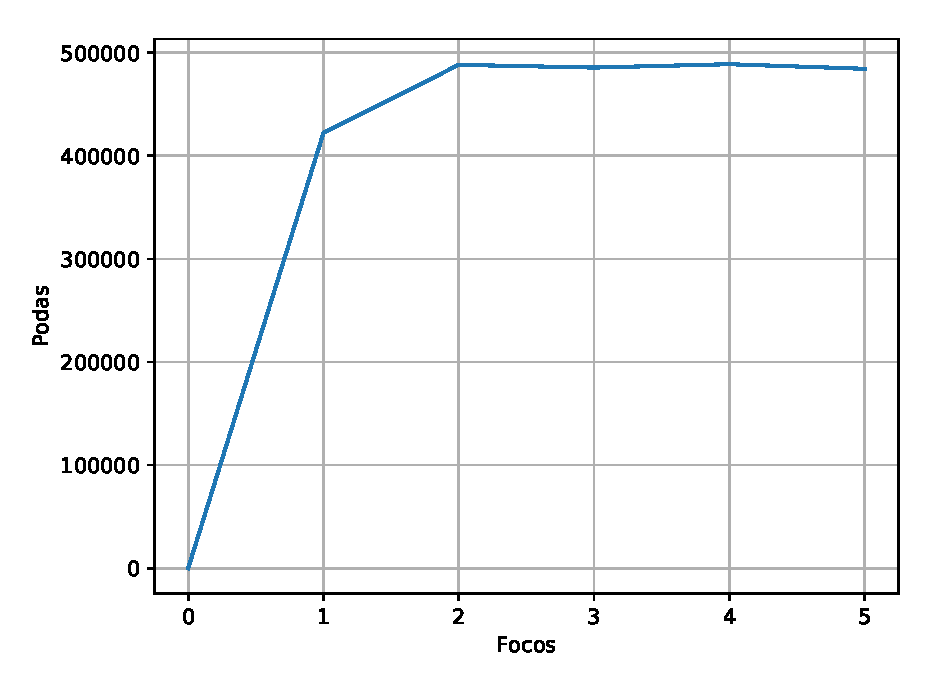
\includegraphics[width=.6\textwidth]{dados/figuras/focoHC.eps}
\fonte{Autoria Própria}
\label{fig:focoHC}
\end{figure}

\begin{figure}[H]
\centering
\caption{Número de podas por focos utilizados para a base cat\_dog}
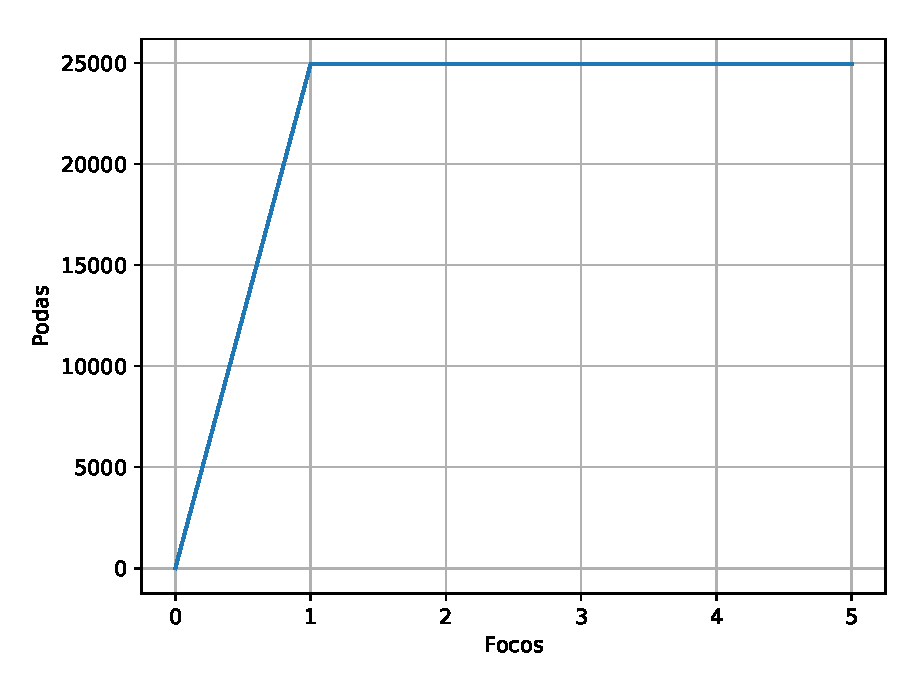
\includegraphics[width=.6\textwidth]{dados/figuras/fococatdog.eps}
\fonte{Autoria Própria}
\label{fig:fococatdog}
\end{figure}

\section{SCRIPTS SQL}
Os scripts necessários para a parte de manipulação do banco de dados foram todos escritos em PLPGSQL, uma linguagem estrutural estendida da SQL, desenvolvida para o uso
no SGBD PostgreSQL. Também foi utilizada a extensão \textit{cube} presente no PostgreSQL, para o cálculo das distâncias. Aqui serão discutidos apenas alguns scripts mais importantes para a análise de resultados. Os demais códigos encontram-se integralmente
nos Apêndices \ref{chap:apendice}. Para fins de otimização dos scripts (tanto sequenciais ou OMNI), tornou-se necessário
a criação de uma função para cada par (atributo, distância) envolvendo a base de dados cat\_dog.

\subsection{SCRIPTS SEQUENCIAIS}
Os scripts sequenciais das consultas realizam a pesquisa vasculhando toda a base de dados, e retornando os elementos que fazem
parte do critério de seleção, seja dentro do raio de abrangência indicado, ou dentre os $k$ elementos mais próximos do elemento central.
Abaixo, códigos utilizados para consultas sequenciais na base cat\_dog.

\begin{lstlisting}[caption={Consulta por abrangência sequêncial utilizando forma e distância euclidiana\\}, captionpos=t,basicstyle=\tiny] 
CREATE OR REPLACE FUNCTION rangeQueryShapeL2 (center_id integer, radius FLOAT8) 
RETURNS SETOF genericQuery AS $$
BEGIN
	  RETURN QUERY SELECT DISTINCT * FROM 
	  (SELECT T2.id_ft, (cube(T1.feature) <-> cube(T2.feature)) AS dist -- <-> indica calculo de
	  FROM SHAPE T1, SHAPE T2 WHERE T1.id_ft = center_id) 		    -- distancia L2
	  AS quer WHERE dist <= radius ORDER BY dist;	
END;$$
LANGUAGE PLPGSQL;
\end{lstlisting}

\begin{lstlisting}[caption={Consulta k-vizinhos mais próximos sequêncial utilizando cor e distância city-block}, captionpos=t,basicstyle=\tiny]
CREATE OR REPLACE FUNCTION kNNColorL1 (center_id integer, k_neigh integer) 
RETURNS SETOF genericQuery AS $$
BEGIN
	RETURN QUERY SELECT * FROM 
	(SELECT T2.ID_FT, (cube(T1.feature) <#> cube(T2.feature)) AS dist  -- <#> indica calculo de 
	FROM COLOR T1, COLOR T2 WHERE T1.id_ft = center_id 		   -- distancia L1
	AND T1.ID_FT <> T2.ID_FT) as quer 
	ORDER BY dist LIMIT k_neigh;	
END;$$
LANGUAGE PLPGSQL;
\end{lstlisting}

Como a base HC apresenta apenas um grande vetor como característica, foram necessárias apenas 3 funções, uma para cada distância Minkowski utilizada.

\begin{lstlisting}[caption={Consulta por abrangência sequêncial utilizando distância Chebyshev para a base HC}, captionpos=t, basicstyle=\tiny]
CREATE OR REPLACE FUNCTION rq_HC_LInf (center_id integer, radius FLOAT8) 
RETURNS SETOF genericQuery AS $$
BEGIN
	RETURN QUERY SELECT DISTINCT * FROM 
	(SELECT T2.COD, (cube(T1.feature) <=> cube(T2.feature)) AS dist   -- <-> indica calculo de
	FROM HC_TABLE T1, HC_TABLE T2 WHERE T1.cod = center_id) as quer   -- distancia LInfinite
	WHERE dist <= radius ORDER BY dist;		
END;$$
LANGUAGE PLPGSQL;
\end{lstlisting}

\subsection{SCRIPTS OMNI}
Para um melhor uso do ganho de desempenho proposto pela técnica OMNI, observou-se a necessidade de criação de uma função para cada tripla (atributo, distância, número de focos). Isto se deve ao fato de que funções em SQL que possuem
o nível de flexibilidade necessário para a passagem de parâmetros como atributo, distância e número de focos utilizados, apresentam uma performance muito inferior quando comparadas com as suas versões \textit{hard-coded}. Além disso, a técnica OMNI
exige uma preparação inicial do banco e a criação das suas estruturas, como mencionado na Seção \ref{sec:tiposconsultas}. Os scripts necessários para essa preparação encontram-se no Apêndice \ref{chap:apendice}. Abaixo, códigos utilizados para 
as consultas OMNI.

\begin{lstlisting}[caption={rangeOmni utilizando 1 foco para a base cat\_dog}, captionpos=t, basicstyle=\tiny, label=code:omni1]
CREATE OR REPLACE FUNCTION rangeOmniShapeL2F1 (center_id integer, radius FLOAT8) 
RETURNS SETOF genericQuery AS $$
DECLARE rec_id RECORD; feature_aux FLOAT8[]; distance FLOAT8; dist_fc FLOAT8;
BEGIN
	SELECT T1.feature INTO feature_aux FROM Shape T1 WHERE T1.id_ft = center_id;
	SELECT dist_l2 INTO dist_fc FROM SHAPE_F_BASE where id_feature = center_id;	
	FOR rec_id IN SELECT id_feature FROM SHAPE_F_BASE 
	WHERE ((dist_l2 < (radius + dist_fc)) AND (dist_l2 > dist_fc - radius)) LOOP
	  SELECT (cube(feature_aux) <-> cube(feature)) 
	  INTO distance FROM SHAPE T1 
	  WHERE rec_id.id_feature = T1.id_ft ;
	  IF (distance < radius) THEN
	    RETURN NEXT (rec_id.id_feature, distance);			       
	  END IF;				
	END LOOP;
END;$$
LANGUAGE PLPGSQL;
\end{lstlisting}

Alguns elementos importantes do Código \ref{code:omni1} requerem uma explanação. Na linhas 3 nota-se a criação de variáveis para o armazenamento de alguns dados lidos. Isto é necessário para armazenar informações importantes
para a consulta em memória, evitando assim o acesso desnecessário a disco que é mais custoso que o acesso à memória. A linha 8 é a responsável pela checagem da pertinência à \textit{mbOr}, 
dada pela desigualdade triangular indicada pela Equação \ref{eq:omnirq}. Da linha 9 até a linha 13 nota-se a etapa de refinamento da técnica, necessária para eliminar elementos que não fazem parte do conjunto-resposta.

Códigos que utilizam mais de um foco apresentam a mesma estrutura, sendo a única diferença a interseção das múltiplas regiões, necessitando $l$ comparações de desigualdade triangular, sendo $l$ o número de focos da base. Essa diferença
é ilustrada na linha 10 do Código \ref{code:omni2}.
\begin{minipage}{\textwidth}
\begin{lstlisting}[caption={rangeOmni utilizando 2 focos para a base HC}, captionpos=t, basicstyle=\tiny, label=code:omni2]
CREATE OR REPLACE FUNCTION rangeOmniHCL2F2 (center_id integer, radius FLOAT8) 
RETURNS SETOF genericQuery AS $$
DECLARE rec_id RECORD; feature_aux FLOAT8[]; distance FLOAT8; dist_fc FLOAT8[];
BEGIN
      SELECT T1.feature INTO feature_aux FROM HC_TABLE T1 WHERE T1.cod = center_id;
      dist_fc = ARRAY(SELECT DISTINCT dist_l2 FROM HC_F_BASE WHERE id_feature = center_id); 
      FOR rec_id IN SELECT id_feature FROM HC_F_BASE 
      WHERE ((dist_l2 < (radius + dist_fc[1])) 
      AND (dist_l2 > dist_fc[1] - radius)) 
      INTERSECT (SELECT id_feature FROM HC_F_BASE 
      WHERE ((dist_l2 < (radius + dist_fc[2])) 
      AND (dist_l2 > dist_fc[2] - radius))) LOOP
	      SELECT (cube(feature_aux) <-> cube(feature)) INTO distance 
	      FROM HC_TABLE T1 WHERE rec_id.id_feature = T1.cod ;
	      IF (distance < radius) THEN
		      RETURN NEXT (rec_id.id_feature, distance);			       
	      END IF;				
      END LOOP; 
END;$$
LANGUAGE PLPGSQL;
\end{lstlisting}
\vspace{0.2cm}
\end{minipage}

\section{TEMPOS DE CONSULTAS}
\label{sec:temp_cons}
Os tempos de consultas foram extraídos como explicados na Seção \ref{sec:metricas}. Os resultados foram obtidos através de uma média de 10 medições distintas, os valores dos centros de pesquisa foram escolhidos aleatoriamente antes
do início dos testes, e o mesmo valor de centro foi utilizado para melhor comparação dos resultados. É importante ressaltar que diferentes características como textura, cor e forma não apresentam alterações significativas
nos tempos de consulta. A Tabela \ref{tab:cd_range_l1} mostra os resultados obtidos para a base CAT\_DOG, com $S_q$ = 42412, $\xi$ = 100 e utilizando a característica de forma.

\begin{table}[!htb]
    \centering
    \caption[Busca por abrangência - CAT\_DOG - L1 - FORMA]{Busca por abrangência - CAT\_DOG - L1 - FORMA.
    \label{tab:cd_range_l1}}
   % \begin{tabular}{l l l l}
   \begin{tabular}{l c c c}
        \midrule
            &Tempo de Execução(ms)&Nº Podas de Cálculos\\
        \midrule
            Sequencial & 8,721 & - \\
            OMNI 1 Foco & 1,747 & 24935 \\
            OMNI 2 Focos & 5,201 & 24935 \\
            OMNI 3 Focos & 7,606 & 24935 \\
            OMNI 4 Focos & 10,107 & 24935 \\
            OMNI 5 Focos & 12,271 & 24935 \\
        \bottomrule
    \end{tabular}
\end{table}

É possível notar que a melhor performance foi obtida com o número ótimo de focos ilustrado pela Figura \ref{fig:fococatdog}. E isto também
pode ser observado nas Tabelas \ref{tab:cd_range_l2} e \ref{tab:cd_range_linf}, que contém os resultados do mesmo experimento anterior, mas para as distâncias
$L_2$ e $L_{\infty}$.

\begin{table}[H]
    \centering
    \caption[Busca por abrangência - CAT\_DOG - L2 - FORMA]{Busca por abrangência - CAT\_DOG - L2 - FORMA.
    \label{tab:cd_range_l2}}
   % \begin{tabular}{l l l l}
   \begin{tabular}{l c c c}
        \toprule
            &Tempo de Execução(ms)&Nº Podas de Cálculos\\
        \midrule
            Sequencial & 8,728 & - \\
            OMNI 1 Foco & 1,825 & 24935 \\
            OMNI 2 Focos & 4,988 & 24935 \\
            OMNI 3 Focos & 7,525 & 24935 \\
            OMNI 4 Focos & 8,994 & 24935 \\
            OMNI 5 Focos & 11,591 & 24935 \\
        \bottomrule
    \end{tabular}
\end{table}

\begin{table}[H]
    \centering
    \caption[Busca por abrangência - CAT\_DOG - L$_\protect\infty$ - FORMA]{Busca por abrangência - CAT\_DOG - L$_\protect\infty$ - FORMA.
    \label{tab:cd_range_linf}}
   % \begin{tabular}{l l l l}
   \begin{tabular}{l c c c}
        \toprule
            &Tempo de Execução(ms)&Nº Podas de Cálculos\\
        \midrule
            Sequencial & 8,805 & - \\
            OMNI 1 Foco & 2,051 & 24935 \\
            OMNI 2 Focos & 4,638 & 24935 \\
            OMNI 3 Focos & 8,563 & 24935 \\
            OMNI 4 Focos & 9,651 & 24935 \\
            OMNI 5 Focos & 11,626 & 24935 \\
        \bottomrule
    \end{tabular}
\end{table}

Outro fator a ser notado é o número de podas permaneceu constante independente do tipo de distância utilizada. Isto se deve ao fato
do valor das distâncias não variarem muito com diferentes distâncias Minkowski para esta base de dados. As Tabelas \ref{tab:cd_range_text} e \ref{tab:cd_range_color}
exemplificam o fato de que diferentes características utilizadas não alteram significativamente a performance
das consultas, como dito no início da Seção \ref{sec:temp_cons}. Para essa consulta, foram utilizados $S_q$ = 42413 e 42414 (característica de
textura e cor referente a mesma imagem da característica de forma com identificador = 42412) e $\xi$ = 100.

\begin{table}[H]
    \centering
    \caption[Busca por abrangência - CAT\_DOG - L1 - TEXTURA]{Busca por abrangência - CAT\_DOG - L1 - TEXTURA.
    \label{tab:cd_range_text}}
   % \begin{tabular}{l l l l}
   \begin{tabular}{l c c c}
        \toprule
            &Tempo de Execução(ms)&Nº Podas de Cálculos\\
        \midrule
            Sequencial & 8,710 & - \\
            OMNI 1 Foco & 1,531 & 24950 \\
            OMNI 2 Focos & 4,512 & 24950 \\
            OMNI 3 Focos & 6,838 & 24950 \\
            OMNI 4 Focos & 9,447 & 24950 \\
            OMNI 5 Focos & 11,182 & 24950 \\
        \bottomrule
    \end{tabular}
\end{table}

\begin{table}[H]
    \centering
    \caption[Busca por abrangência - CAT\_DOG - L1 - COR]{Busca por abrangência - CAT\_DOG - L1 - COR.
    \label{tab:cd_range_color}}
   % \begin{tabular}{l l l l}
   \begin{tabular}{l c c c}
        \toprule
            &Tempo de Execução(ms)&Nº Podas de Cálculos\\
        \midrule
            Sequencial & 8,334 & - \\
            OMNI 1 Foco & 1,675 & 24923 \\
            OMNI 2 Focos & 4,819 & 24923 \\
            OMNI 3 Focos & 8,073 & 24923 \\
            OMNI 4 Focos & 9,628 & 24923 \\
            OMNI 5 Focos & 12,925 & 24923 \\
        \bottomrule
    \end{tabular}
\end{table}

Para a base HC, também é possível verificar o ganho de performance obtido pela técnica OMNI. Como a base é significativamente maior e os dados mais complexos, o ganho
de performance é mais notável, como ilustram as Tabelas \ref{tab:hc_range} e \ref{tab:hc_range2}. Estas tabelas foram construídas utilizando consultas com $S_q$ = 49628 e $\xi$ = 20.
Novamente, a melhor performance pode ser observada com o número ótimo de focos indicado pela Figura \ref{fig:focoHC}.

\begin{table}[H]
    \centering
    \caption[Busca por abrangência - HC- L1]{Busca por abrangência - HC - L1.
    \label{tab:hc_range}}
   % \begin{tabular}{l l l l}
   \begin{tabular}{l c c c}
        \toprule
            &Tempo de Execução(ms)&Nº Podas de Cálculos\\
        \midrule
            Sequencial & 4566,851 & - \\
            OMNI 1 Foco & 448,105 & 484381 \\
            OMNI 2 Focos & 292,709 & 490599 \\
            OMNI 3 Focos & 361,712& 499406 \\
            OMNI 4 Focos & 462,795 & 499845 \\
            OMNI 5 Focos & 882,159 & 499937 \\
        \bottomrule
    \end{tabular}
\end{table}

\begin{table}[H]
    \centering
    \caption[Busca por abrangência - HC- L2]{Busca por abrangência - HC - L2.
    \label{tab:hc_range2}}
   % \begin{tabular}{l l l l}
   \begin{tabular}{l c c c}
        \toprule
            &Tempo de Execução(ms)&Nº Podas de Cálculos\\
        \midrule
            Sequencial & 4310,409 & - \\
            OMNI 1 Foco & 1215,435 & 422246 \\
            OMNI 2 Focos & 307,757 & 484381 \\
            OMNI 3 Focos & 556,683 & 485574 \\
            OMNI 4 Focos & 598,664 & 488229 \\
            OMNI 5 Focos & 952,008 & 488841 \\
        \bottomrule
    \end{tabular}
\end{table}

A técnica OMNI aplicada com a consulta por $k$-vizinhos mais próximos não conseguiu trazer resultados mais rápidos do que a
consulta sequencial. Isto se deve ao fato de que esta consulta efetua uma busca por abrangência em torno do elemento central de pesquisa, e 
retorna os $k$ valores mais próximos. Para isto, o valor do raio utilizado deve ser grande o bastante para retornar um número razoável
de elementos. O Código \ref{code:knnomni} ilustra como foram feitas as consultas OMNI-\textit{kNN}.
\begin{minipage}{\textwidth}
\begin{lstlisting}[caption={kNN-OMNI utilizando 2 focos para a base HC}, captionpos=t, basicstyle=\tiny, label=code:knnomni]
CREATE OR REPLACE FUNCTION kNNOmniHCL2F2 (center_id INTEGER, k_value INTEGER) 
RETURNS SETOF genericQuery AS $$
DECLARE radius FLOAT8 := 100;
BEGIN
	RETURN QUERY SELECT * 
	FROM rangeOMNIHCL2F2(center_id,radius) 
	ORDER BY distance LIMIT k_value;		
END;$$
LANGUAGE PLPGSQL; 
\end{lstlisting}
\vspace{2cm}
\end{minipage}

Outra forma implementada foi a expansão do raio em tempo de execução da consulta, caso seja pequeno demais para retornar
os $k$ elementos necessários, mas este método provou ser ainda menos eficiente que o previamente mencionado. A Tabela \ref{tab:knnHC}
contém os valores dos tempos de execução de uma consulta OMNI-\textit{kNN} com $s_q$ = 75003, $k$ = 30. O valor de $\xi$ utilizado para
efetuar a consulta foi de 100.


\begin{table}[H]
    \centering
    \caption[Busca OMNI-\textit{kNN} - HC- L2]{Busca OMNI-\textit{kNN} - HC - L2.
    \label{tab:knnHC}}
   % \begin{tabular}{l l l l}
   \begin{tabular}{l c c }
        \toprule
            &Tempo de Execução(ms)\\
        \midrule
            Sequencial & 4733,579  \\
            OMNI 1 Foco & 6519,995  \\
            OMNI 2 Focos & 6341,987  \\
            OMNI 3 Focos & 7490,256 \\
            OMNI 4 Focos & 7548,550 \\
            OMNI 5 Focos & 10348,541 \\
        \bottomrule
    \end{tabular}
\end{table}

O uso da distância $L_\infty$ na base de dados HC provou ser inviável. A distância Minkowski com $p = \infty$ essencialmente mede a 
maior diferença de valores entre duas dimensões quaisquer de dois pontos. Como a base possui os valores dos seus atributos entre 0 e 256, 
esta distância geralmente convergia para 256, tornando boa parte da base igualmente espaçada entre si, e entre os focos. Isto dificulta
a poda de elementos, tornando a técnica ineficaz nesta situação.

\section{ANÁLISE QUALITATIVA DAS CONSULTAS}

As consultas tanto sequenciais como OMNI retornam o mesmo resultado, sendo a diferença apenas a velocidade de execução da consulta. O foco deste trabalho
mantém-se apenas nos tempos das consultas, mas para ilustrar como seriam o retorno dessas consultas, seguem abaixo alguns exemplos
de consultas nas três características da base CAT\_DOG.

\begin{figure}[H]
  \centering
  \subfloat[cat.50 - $S_q$]{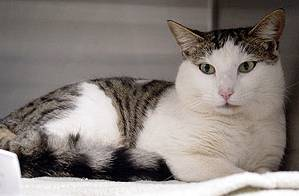
\includegraphics[width=.20\textwidth]{dados/figuras/cat50.jpg}} \hspace{2cm}
  \subfloat[cat.9211]{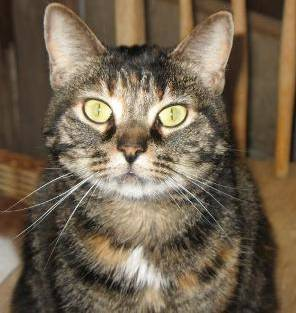
\includegraphics[width=.20\textwidth]{dados/figuras/cat9211.jpg}} \hspace{2cm}
  \subfloat[dog.10089]{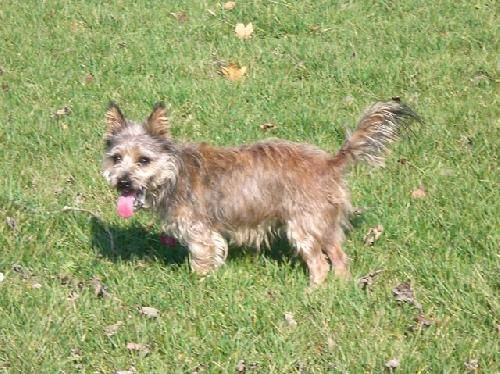
\includegraphics[width=.20\textwidth]{dados/figuras/dog10089.jpg}}\\
  \subfloat[dog.3125]{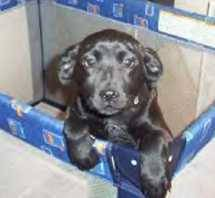
\includegraphics[width=.20\textwidth]{dados/figuras/dog3125.jpg}} \hspace{2cm}
  \subfloat[cat.5010]{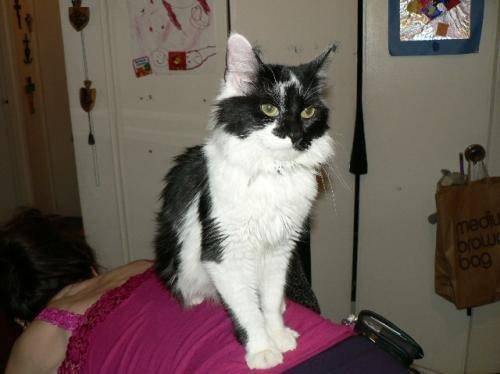
\includegraphics[width=.20\textwidth]{dados/figuras/cat5010.jpg}} \hspace{2cm}
  \subfloat[cat.4258]{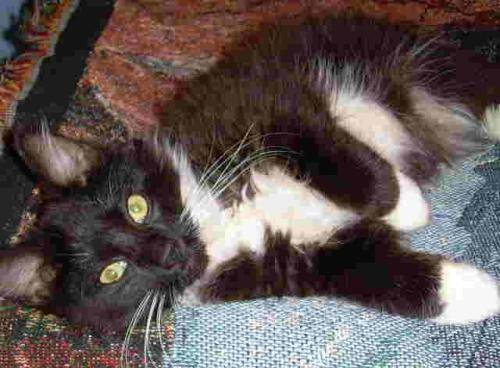
\includegraphics[width=.20\textwidth]{dados/figuras/cat4258.jpg}} \\
  \caption{Exemplo de consulta por abrangência utilizando Forma}
\end{figure}

\begin{figure}[H]
  \centering
  \subfloat[dog.6431 - $S_q$]{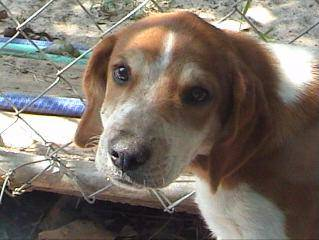
\includegraphics[width=.20\textwidth]{dados/figuras/dog6431.jpg}} \hspace{2cm}
  \subfloat[cat.3864]{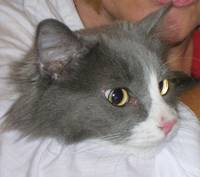
\includegraphics[width=.20\textwidth]{dados/figuras/cat3864.jpg}} \hspace{2cm}
  \subfloat[cat.6114]{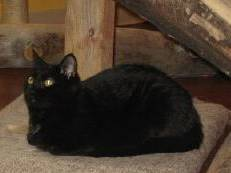
\includegraphics[width=.20\textwidth]{dados/figuras/cat6114.jpg}}\\
  \subfloat[cat.8027]{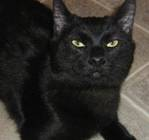
\includegraphics[width=.20\textwidth]{dados/figuras/cat8027}} \hspace{2cm}
  \subfloat[dog.12048]{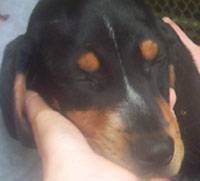
\includegraphics[width=.20\textwidth]{dados/figuras/dog12048.jpg}} \hspace{2cm}
  \subfloat[dog.4639]{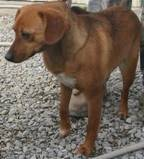
\includegraphics[width=.20\textwidth]{dados/figuras/dog4639.jpg}} \\
  \caption{Exemplo de consulta por abrangência utilizando Textura}
\end{figure}

\begin{figure}[H]
  \centering
  \subfloat[dog.11868 - $S_q$]{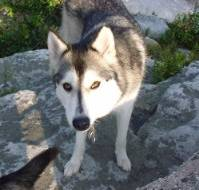
\includegraphics[width=.20\textwidth]{dados/figuras/dog11868.jpg}} \hspace{2cm}
  \subfloat[cat.12219]{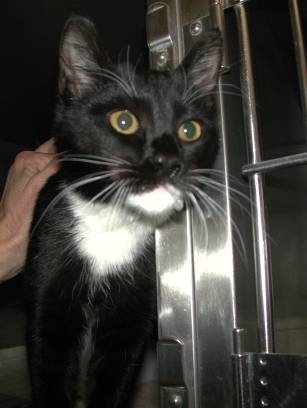
\includegraphics[width=.20\textwidth]{dados/figuras/cat12219.jpg}} \hspace{2cm}
  \subfloat[dog.9322]{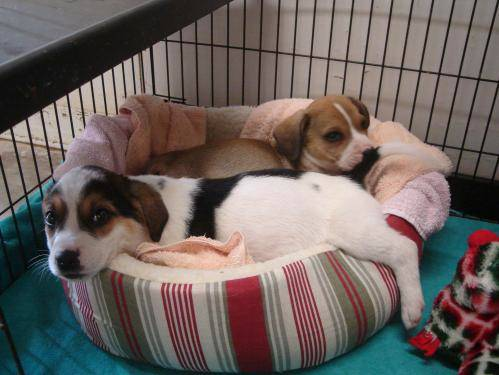
\includegraphics[width=.20\textwidth]{dados/figuras/dog9322.jpg}}\\
  \subfloat[cat.9185]{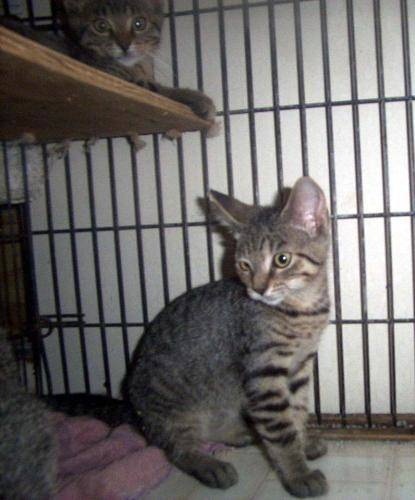
\includegraphics[width=.20\textwidth]{dados/figuras/cat9185}} \hspace{2cm}
  \subfloat[cat.4439]{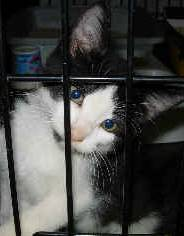
\includegraphics[width=.20\textwidth]{dados/figuras/cat4439.jpg}} \hspace{2cm}
  \subfloat[dog.10028]{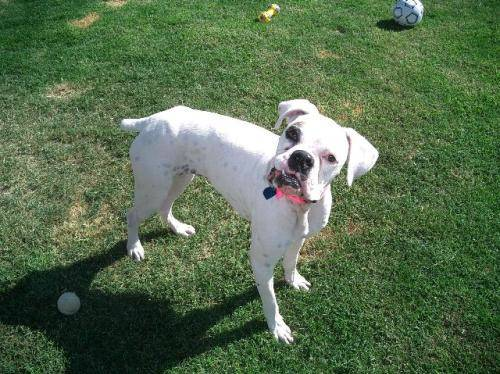
\includegraphics[width=.20\textwidth]{dados/figuras/dog10028.jpg}} \\
  \caption{Exemplo de consulta por abrangência utilizando Cor}
\end{figure}


\section{LIMITAÇÕES DA TÉCNICA}
\label{sec:limit}
Embora a técnica OMNI mostrou-se eficaz para consultas por abrangência mesmo em bases pequenas e com baixo nível de complexidade,
algumas limitações são inerentes à natureza da técnica. A principal limitação é em relação ao tamanho do raio $\xi$ empregado em consultas OMNI.
Quanto maior o raio, menos elementos são descartados pela etapa de poda, sendo necessário mais cálculos de pertinência à \textit{mbOr} e mais cálculos
de distância. As Tabelas \ref{tab:limit1} e \ref{tab:limit2} mostram um comparativo do tempo de execução de consultas por abrangência sequenciais e OMNI conforme aumenta-se
o raio de pesquisa para as bases CAT\_DOG e HC, juntamente com o número de elementos do conjunto resposta.

\begin{table}[H]
    \centering
    \caption[Performance em função do aumento do raio - CAT\_DOG]{Performance em função do aumento do raio - CAT\_DOG.
    \label{tab:limit1}}
   % \begin{tabular}{l l l l}
   \begin{tabular}{c c c c}
        \toprule
           Raio &Sequencial (ms)&OMNI (ms) &Nº Elementos\\
        \midrule
            100 & 8,598 & 1,938 & 62 \\
            500 & 8,580 & 4,582 & 324 \\
            1000 & 8,951 & 7,91 & 633 \\
            1500 & 8,760 & 11,119 & 973 \\
            2000 & 9,164 & 12,735 & 1331 \\
            2500 & 9,518 & 16,379 & 1654 \\
            3000 & 10,307 & 20,153 & 2000 \\
            3500 & 10,466 & 25,228 & 2303 \\
            4000 & 10,464 & 28,088 & 2597 \\
            4500 & 10,609 & 29,088 & 2928 \\
           
        \bottomrule
    \end{tabular}
\end{table}

\begin{table}[H]
    \centering
    \caption[Performance em função do aumento do raio - HC]{Performance em função do aumento do raio - HC.
    \label{tab:limit2}}
   % \begin{tabular}{l l l l}
   \begin{tabular}{c c c c}
        \toprule
           Raio &Sequencial (ms)&OMNI (ms) &Nº Elementos\\
        \midrule
            20 & 4742,696 & 254,221 & 11 \\
            50 & 4917,345 & 1122,165 & 553 \\
            80 & 4626,832 & 1890,589 & 2001 \\
            110 & 4762,850 & 2683,298 & 4256 \\
            140 & 4825,782 & 3531,885 & 7992 \\
            170 & 4708,758 & 8280,403 & 13903 \\
            200 & 4927,518 & 8251,041 & 22708 \\
            230 & 4893,118 & 8393,683 & 36753 \\
            260 & 5157,097 & 8800,501 & 59719 \\
            290 & 5415,949 & 9045,798 & 95710 \\
           
        \bottomrule
    \end{tabular}
\end{table}